\documentclass{article}

\usepackage[final]{nips_2018}
\usepackage[utf8]{inputenc} % allow utf-8 input
\usepackage[T1]{fontenc}    % use 8-bit T1 fonts
\usepackage{hyperref}       % hyperlinks
\usepackage{url}            % simple URL typesetting
\usepackage{booktabs}       % professional-quality tables
\usepackage{amsfonts}       % blackboard math symbols
\usepackage{nicefrac}       % compact symbols for 1/2, etc.
\usepackage{microtype}      % microtypography
\usepackage{amsmath}
\usepackage{float}
\usepackage{graphicx}
\graphicspath{{figures/}{}}

\title{Final project of SLML --- \\Learning to Score Figure Skating Sport Videos}


\author{%
\
}

\begin{document}
% \nipsfinalcopy is no longer used

\maketitle

\begin{abstract}
This article presents a new structure to score figure skating sport video, where our inputs are features of the FisV video extracted by C3D convolutional neural network. To achieve our goal, we devise a Self-attentive Multi-scale LSTM which implements self-attention perspectively in three different parallel scales. This new structure is essentially a exquisite combination of Self-attentive LSTM and multi-scale LSTM, but making up their shortcomings form each other. Specifically, this structure equips our model with the ability to focus on different regions and details on different time scales. Furthermore, we employ two internationally accepted scores, TES and PCS as our aim score, and Mean Square Error and Spearman's correlation between predicted score and real score as our evaluation indexes. This structure shows a great performance in our experiment.
\end{abstract}

\section{Introduction}
Figure skating is a well-known elegant and graceful sports. Thanks to the rapid development of digital cameras and proliferation of social media sharing, figure skating is getting more and more widespread and popular. Bunches of figure skating sports videos are available easily on the internet, including over 20 international figure skating competitions held by International Skating Union (ISU).  However, nearly all the videos just show the performance of the skaters, they do not show the outcome, that is the professional score from the referees. Actually, it is not very convenient for someone to get the scoring record for a exact sports video of one competition. But for whomever watches the videos, they need to know whether the performance is perfect or not objectively, which means we can not always use intuitive feeling about the performance of the skaters.\\ 
So, we aim to score such figure skating performances with only original videos provided. Once we can handle this task accurately enough, we can attach predicted score to each video for viewers This predicted score can be a important reference for viewers, most of whom are amateurs, to learn and appreciate. To achieve this, the given scores should be as detailed as possible, for instance, there are two kinds of scores, TES and PCS(TES assesses technical movements and PCS assesses interpretation of music), provided in our figure skating scoring systems. There is a wide potential application for this intelligent scoring system, as all kinds of sports and our competitions with a performance-score system can apply this scoring system. What's more, the ideas and machine learning method we use to achieve this scoring system can be applied in other more difficult projects. This will be discussed in the following content.
\section{Related Work}
From the basic paper provided in the final project, we have known that the videos are represented by C3D features from a 3D convolutional network.So, predicting the PCS and TES of the figure skating video can be seen as a sequence to sequence `regression' problem, what we need is an encoder for input and a decoder for output.We have looked up many implement methods of encoder-decoder model, and the most famous state-of-the-art model is the Transformer [2], proposed by Google in Nov,2017.The transformer is aimed to deal with issues related to sequential models based on the attention structure. One of the most important content of the paper, `Attention is all you need', is the brand new self-attention structure, which is implied by us in our project and has a wonderful effect.\\
The main structure diagram of the Transformer is shown is in Figure \ref{transformer}.
\begin{figure}[H]
	\centering
	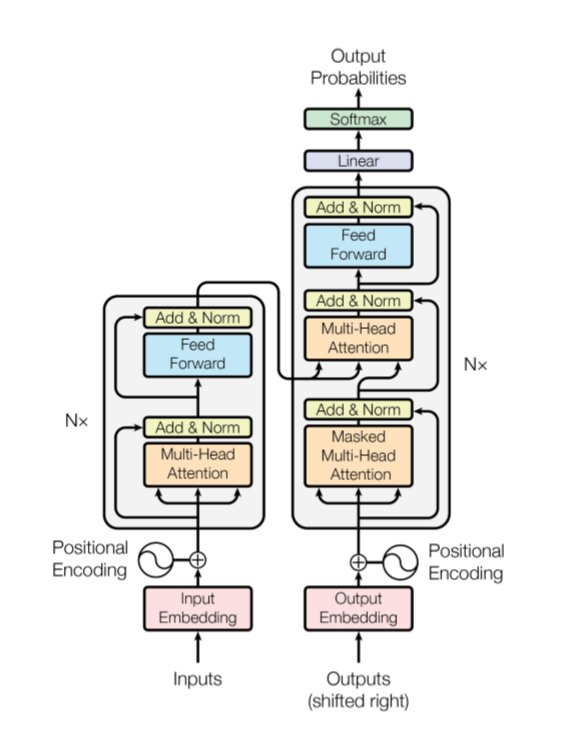
\includegraphics[width=10cm]{transformer}
	\caption{the Transformer}
	\label{transformer}
\end{figure}
The encoder is stacked by six identical layers, each with two more layers. The first support layer is a long self-attention mechanism, and the second support layer is a simple fully connected feedforward network. A residual connection is added outside the two layers, and then layer normalization is performed. All the support layers of the model and the output dimensions of the embedding layer are $d_{model}$s.The decoder is also stacked with six identical layers. However, in addition to the two support layers in the encoder, the decoder also adds a third support layer, as shown in the figure also uses the residual and layer normalization. The input to the encoder and decoder is to convert the token into a dmodel dimension vector using well-known embeddings. For the decoder, the linear transform and the soft-max function are used to convert the decoded output into a probability of predicting the next token.\\
The Transformer uses scaled dot-product attention. Inputs include queries and keys with dimensions $d_{k}$, and values with dimensions $d_{v}$. Calculate the dot multiplication of the query and all keys, and then divide each by $\sqrt{d_{k}}$ (the operation is called Scaled). Then use a soft-max function to get the weight of values. The mathematical expression can be shown as:
\begin{align}
\label{attention}
Attention(Q,K,V)&=softmax(\frac{QK^T}{\sqrt{d_k}})V
\end{align}
Further more, the Transformer uses multi-head attention, that is the Attention in the structure of this article is not simply to apply a point-multiplied attention. It is especially good to perform different linear mappings for queries, keys, and values. The learned linear maps are mapped to $d_{k}$, $d_{k}$, and $d_{v}$ dimensions, respectively. The parallel operation of the attention function is performed on each of the obtained queries, keys and values after each mapping, and the output value of the $d_{v}$ dimension is generated. The specific structure and formula are as follows:
\begin{align}
Multihead(Q,K,V)&=Concat(head_1,\dots,head_h)W^O\\
\label{multihead}
head_i&=Attention(QW_i^Q,KW_i^K,VW_i^V),\quad i=1,\dots,h
\end{align}
The structure of the attention is shown in Figure \ref{attention} and Figure \ref{multi-head attention} .\\
\begin{figure}[H]
	\centering
	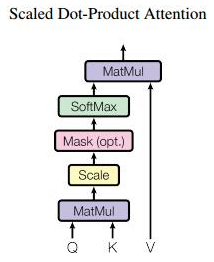
\includegraphics[width=6cm]{attention}
	\caption{Scaled Dot-Product Attention}
	\label{attention}
\end{figure}
\begin{figure}[H]
	\centering
	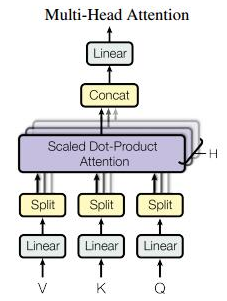
\includegraphics[width=6cm]{mh-attention}
	\caption{Multi-Head Attention}
	\label{multi-head attention}
\end{figure}
In the attention layer of the encoder-decoder, the queries are from the previous decoder layer, and the keys and values are from the output of the encoder. This is similar to the attention mechanism used by many of the proposed seq2seq models. The encoder contains a self-attention layer. In a self-attention layer, all the keys, values, and queries are from the same place, in this case the output of the layer before the encoder. Similarly, the self-attention layer in the decoder is the same. The difference is that the masked point is added to the attention operation by adding a mask operation. This operation is to ensure that the illegal values will not be connected to the attention after the soft-max operation.\\
The other layer after the attention is a feedforward network. The formula is described below.
\begin{align}
\textit{FFN}(x)=\textit{max}(0,xW_{1}+b_{1})W_{2}+b_{2}
\end{align}
In a word, the Transformer framework is very instructive as it abandons CNN and RNN (very frequently-used in deep learning tasks) with self-attention. It makes the training process much faster and what's more, we can get better outcome.

\section{Discussion of Proposed Models}
Inspired by self-attentive LSTM (S-LSTM) and multi-scale convolutional skip LSTM (M-LSTM) in [1] and transformer in [2], we devised a new structure which aims to inherit and merge the advantages of S-LSTM and M-LSTM while overcoming their disadvantages.

\subsection{Analysis and Inspiration}
\label{analysis}
\paragraph*{S-LSTM} In S-LSTM, the author implement the method of self-attention as feature embedding, which was first proposed in Google's work[2] (transformer). But there are several deferences between S-LSTM and transformer:

\begin{itemize}
\item[(1)] Transformer aims to finish the task of sequence to sequence, while the skating scoring task in S-LSTM is a N-to-1 problem.
\item[(2)] Transformer abandoned the thought of RNN, complementing the task only by the mechanism of attention, while S-LSTM make use of self-attention as a means of dimension reduction and embedding and still use RNN (LSTM) to get scores.
\item[(3)] Multi-head attention was used in transformer while single-head attention was used in S-LSTM.
\item[(4)] Layer normalization was applied in transformer while not applied in S-LSTM.
\end{itemize}

In response to these differences, we tried with different improvements in the following part and reported their performance.

\paragraph*{M-SLTM} 
As for the structure of M-LSTM, it uses the idea of GoogLeNet, which also implement multi-scale convolution of different kernel size and stride length, small kernel for local features and big kernel for global ones. In order to illustrate where our inspiration comes from, we also list our the deferences between GoogLeNet and M-LSTM here.

\begin{itemize}
\item[(1)] The convolution operation in GoogLeNet is applied in the dimensions of space while in the dimension of time in M-LSTM. In other words, GoogLeNet uses convolution to extract the local and global features in different regions of the video, while M-LSTM uses it to extract patterns through time (in several seconds).
\item[(2)] GoogLeNet stacks the output of convolutional layers of different kernels and strides in depth (stack as channels). M-LSTM concatenates different output from Skip-LSTM.
\item[(3)] No pooling layer in M-LSTM.
\item[(4)] No attention mechanism in M-LSTM.
\end{itemize}

We should notice that actually difference (2) doesn't make sense, since the tensor of the output in convolutional layer are often concatenated into a vector before connecting to fully-connected layer.

\subsection{Proposed Structures and Experiments}
\label{structure}
Firstly, we modified S-LSTM and then M-LSTM perspectively according to the analysis above. Finally, we devised a new structure based on M-LSTM and S-LSTM which outweighs both of them.
\subsubsection{Multi-head attention}
We tried with multi-head attention proposed in transformer to modify S-LSTM, which are shown in Eq (\ref{attention})$\sim$(\ref{multihead}).

The output of (\ref{multihead}) are put into a LSTM then a fully connected layer with activation function to regress the PCS and TES score.
The results are terrible, with Spearman correlation of only about 0.5 for both TES and PCS. As a general setting, we choose $h=8$ parallel attention layers so $d_k=d_v=d_{model}/h=512$. Besides, key-value pairs are set as $K=V$ here.\par
The bad performance may come from two main reasons:

\begin{itemize}
\item[(1)] Multi-head attention in [1] are designed for sequence-to-sequence problem and structure without RNN.
\item[(2)] There is also probability that multi-head attention focuses on redundant features, thus giving them relative high weights.
\end{itemize}

\subsubsection{Layer Normalization}
We add a layer normalization[3] between the output of the LSTM layer and the fully connected layer to decrease the risk of overfitting.From [3],we know that layer normalization is designed to overcome the drawbacks of batch normalization. When doing layer normalization, we fix the mean and the variance of the summed inputs within each layer as follows:
\begin{align}
\mu^{l}=\frac{1}{H}\Sigma^{H}_{i=1}a_{i}^{l}\\
\sigma^{l}=\sqrt{\frac{1}{H}\Sigma^{H}_{i=1}(a_{i}^{l}-\mu^{l})^{2}}
\end{align}
where H denotes the number of hidden units in a layer.\\
In deep neural networks,Notice that changes in the output of one layer will tend to cause highly correlated changes in the summed inputs to the next layer(especially with ReLU units whose outputs can change by a lot),this is called `covariate shift' problem.This problem can be reduced by fixing the mean and the variance of the summed inputs within each layer to the above form(layer normalization).Under layer normalization, all the hidden units in a layer share the same normalization terms $\mu$ and $\sigma$,but different training cases have different normalization terms.Unlike batch normalization, layer normalization does not impose any constraint on the size of a mini-batch.


\subsubsection{Bi-directional LSTM}
For S-LSTM, apart from structure mentioned above, we also tried other structures such as the bi-directional LSTM, which includes a forward process and a backward process through time:

\begin{align}
Forward:\quad h_t&=f(W_1x_t+W_2h_{t-1})\\
Backward:\quad h_t'&=f(W_3x_t+W_5h_{t+1}')\\
Output:\quad o_t&=g(W_4h_t+W_6h_t')
\end{align}

Expectedly, it performed badly, because when watching skating competitions attentively, we didn't have sufficient time to recall previous performance. So it's mainly a forward process, not a bi-directional one.\par

\subsubsection{Multi-scale Convolution in Features}
We tried to expand the convolutional kernel in M-LSTM not only in the dimension of time, but also in the dimension of features. It didn't work and Spearman's correlation between given scores and predicted scores declined.\par
The reason for it is simple: the input features are extracted by C3D convolutional neural network and put into a vector of length 4096. The spacial structure of each frame were destroyed during the process of extracting features and stretching into a vector. So we cannot continue doing convolution on the feature vectors.

\subsection{Our Final Model: Self Attentive Multi-scale LSTM (SM-LSTM)}
According to our analysis in \ref{analysis} and experiments in \ref{structure}, we could get to know that the most significant shortcoming for S-LSTM and M-LSTM is that:\par

\textbf{S-LSTM} lacks multi-head attention but we can't add it directly. To some degree, what it really lacks is the idea of diversity in a model.\par
\textbf{M-LSTM} lacks attention mechanism which could focus the attention of the model on important parts of features and as a result, perform dimension reduction.\par

Coincidently, M-LSTM is abundant in what S-LSTM lacks, i.e. diversity. The multi-scale convolutional kernel in M-LSTM provides the model with diversity in different time scales. And simultaneously, S-LSTM could make up the attention mechanism that M-LSTM shorts for.\par
This could also explain why S-LSTM+M-LSTM has did a good job in predicting skating scores. More importantly, it inspires us to combine M-LSTM with S-LSTM to produce a new structure, which was shown in Figure \ref{SM-LSTM}.\par

Firstly, we compute different self-attention for different scale, then multiply with our feature matrix perspectively:

\begin{align}
A_i &= softmax\left(W_{s2,i}tanh\left(W_{s1,i}F^T\right)\right), \quad i=1,2,3\\
M_i &= A_iF, \quad i=1,2,3
\end{align}
where weights matrix $W_{s1,i}(d_1\times d), W_{s2,i}(d_2\times d_1),i=1,2,3$ are determined from learning.\par

This structure equips our model with the ability of different focus points in different time scale, since each row of attention matrix A can be interpreted as a measure of importance (normalized by softmax, sum to 1) for time vector of length $T$. After these process, we get $d_2\times T$ matrices $M_i, i=1,2,3$. Note that different from transformer and the same to S-LSTM, we use matrix product here instead of dot product for the sake of dimension reduction. After these process, feature dimension $d$ has been reduced to $d_2$, which is far more less than $d$, so it also serve as an embedding layer.\par

Then, matrix $M_i$ was put into an LSTM of $256$ neurons (128 neurons for the LSTM on the bottom) to get the last output. Here we abandoned Skip-LSTM which could accelerate training by skipping redundant information, for the reason that we have already implemented self-attention to give different weights for each feature in each frame, which would allocate small weights for unimportant information.\par

\begin{figure}[H]
	\centering
	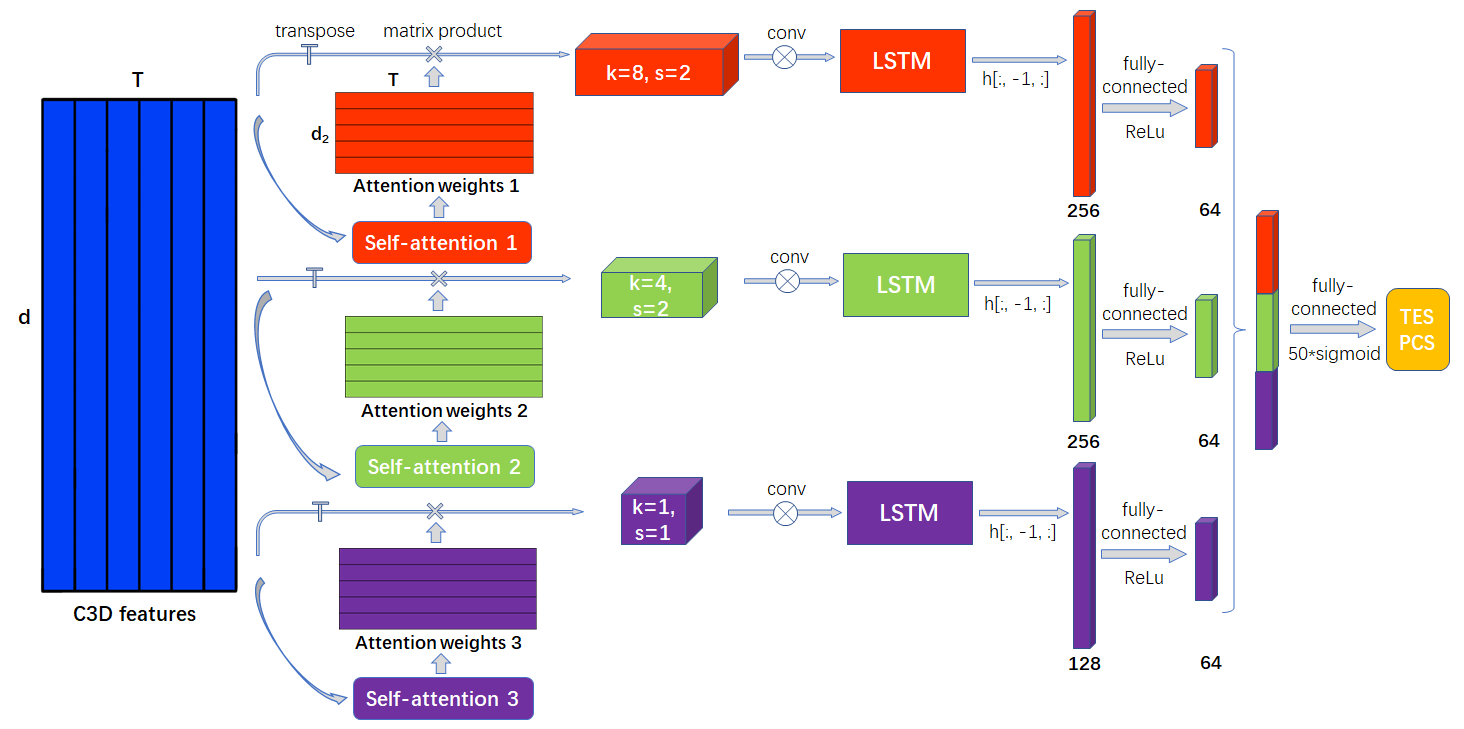
\includegraphics[width=16cm]{SM-LSTM}
	\caption{Self-attentive multi-scale LSTM.}
	\label{SM-LSTM}
\end{figure}

Additionally, it should be stressed that this model actually includes a weighted S-LSTM. Notice the bottom row of figure \ref{SM-LSTM} (the purple parts), a convolutional kernel of size $1$ and stride $1$ is essentially a constant product term, so it's the same as a S-LSTM multiplying a constant. The trick is that we merged this S-LSTM into M-LSTM as a parallel layer of multi-scale.

The last output of LSTM, a vector of length $256$ was taken out and put into a fully-connected layer with activation function ReLu to get a vector of length $64$. Concatenate the $3$ vectors and implement another fully-connected layer with activation function of $50\times sigmoid$ to regress predicted TES and PCS.

\begin{align}
V_{h,i}&=LSTM(M_i \ast kernel_i), \quad i=1,2,3\\
V_{fc,i}&=ReLu(W_{fc,i}V_{h,i}), \quad i=1,2,3\\
V_{cat}&=concat(V_{fc,1},V_{fc,2},V_{fc,3})\\
[TES,PCS]&=50\times sigmoid(W_OV_{cat})
\end{align}
where $\ast$ represents for convolution.\par

We choose ReLu as the activation function of the first fully-connected layer to add some non-linearity. The second activation function are set as $50\times sigmoid$ to assure that the all the output values are in the range of $(0,50)$ because it's nearly impossible to get a score more than 50 though no limit to the highest score in figure skating. What's more, the empirical cumulative density function (CDF) of TES/PCS and sigmoid are shown in Figure \ref{sigmoid}. We can see that most of the scores are in the middle section and extreme scores are rare. And sigmoid function which can hardly get extreme low or high values satisfies this requirement. And obviously, the difference between empirical cumulative function of TES/PCS and sigmoid is only a bias in the horizontal axis, which can be leant in the bias term of the fully-connected layer. Therefore, we have sufficient confidence to employ $50\times sigmoid$ as the activation function of the last fully-connected layer.

\begin{figure}[H]
	\centering
	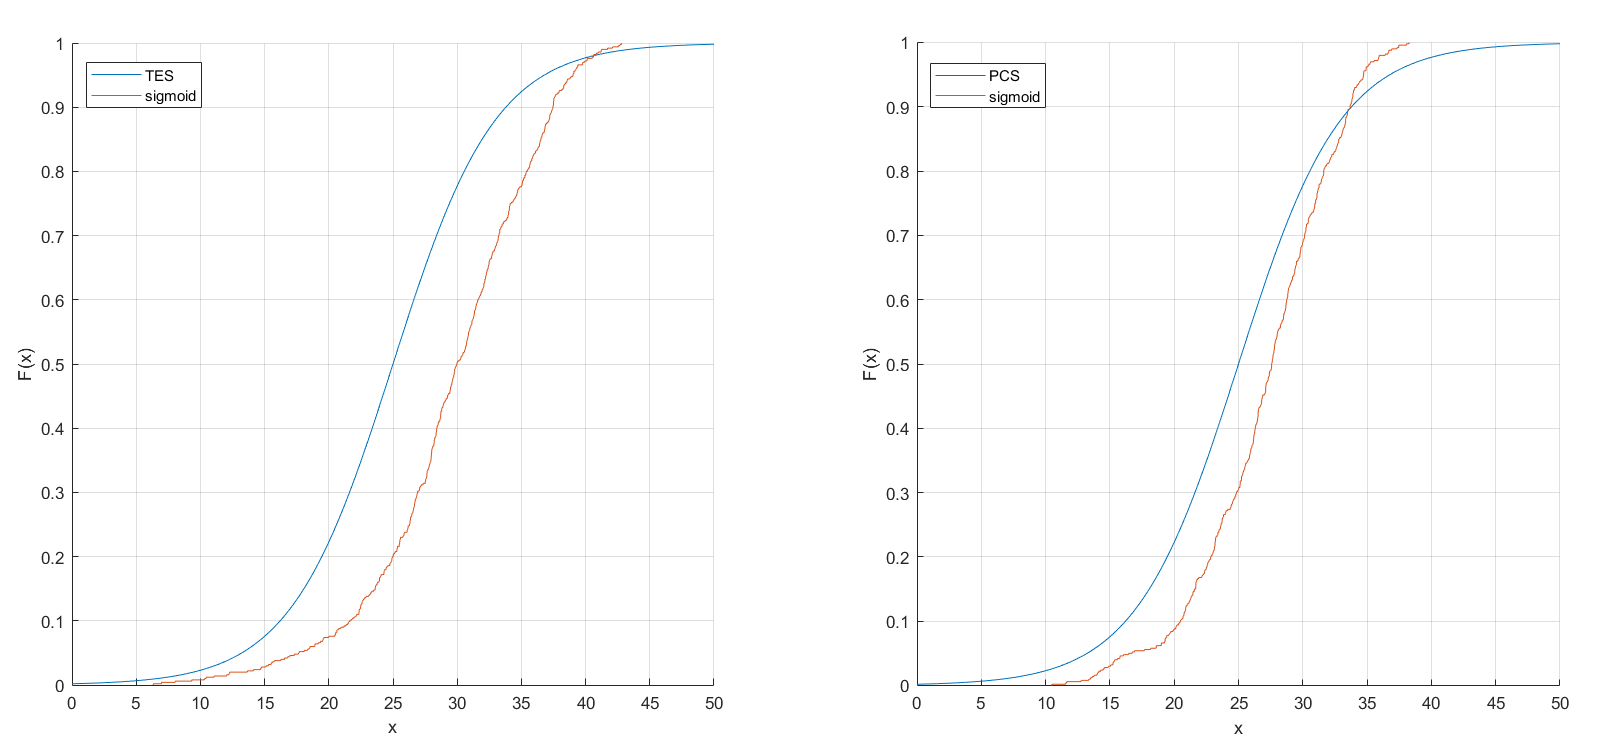
\includegraphics[width=14cm]{sigmoid}
	\caption{Comparison of sigmoid and empirical cumulative density function of TES (left) and PCS (right).}
	\label{sigmoid}
\end{figure}


\section{Experiments of SM-LSTM}
\subsection{Loss function}
The loss function was constructed in the same manner of [1] expect for an extra constant multiplier $\beta$ on the penalty term, which penalize the correlation between self-attentive features, and adjusts the trade-off between diversity of self-attention and accuracy of the model (bias-variance trade-off):

\begin{align}
penalty:\quad P_i&=\Vert AA^T-I \Vert_F^2,\quad i=1,2,3\\
loss:\quad L&=MSE(TES, TES_{pred})+MSE(PCS, PCS_{pred})+\beta(P_1+P_2+P_3)
\end{align}
where $\Vert\cdot\Vert_F^2$ is squared Frobenius norm and MSE stands for mean square error.

\subsection{Preprocessing}
There is a problem that all the feature matrices have different length of time, so we should do some preprocessing to make them the same shape. We tried with forward zero-padding (pad zeros before shorter sequence) and backward zero-padding (pad zeros after shorter sequence). The results in our experiments indicates that forward zero-padding is better.

\subsection{Capped Gradient}
Another small trick was used in our training: we capped all the gradients to the range of $[-a,a]$ to avoid violent shake caused by enormous gradient in the beginning of training. This trick is a little like warm-up which implement small learning rate at the beginning of training. We didn't use warm-up for we have already used Adam to manage our training. In our experiment, hyper-parameter $a$ is set to be $5$.


\subsection{Parameters}
In correspond to our SM-LSTM model, we use tensorflow to construct our model and adjust hyper-parameters in it. Dropout are implemented in each fully-connected layer. And the best parameters according to our experiments are shown as follows:

\begin{table}[H]
	\centering
	\caption{Adjusted hyper-parameters.}
	\label{parameter}
	\begin{tabular}{cccccccc}
	\toprule
	learning rate $\alpha$ & epoch & batch size & drop out & $d_1$ & $d_2$ &  $beta$  & optimizer\\
	\midrule
	      $10^{-4}$        &  300  &     32     &    0.5   &  512  &    40   & $10^{-2}$ &  Adam \\
	\bottomrule
	\end{tabular}
\end{table}


\section{Results and Analysis}
We report the results of Spearman correlation in table 2.
\begin{table}[H]
  \caption{Results of Spearman correlation}
  \label{sc}
  \centering
  \begin{tabular}{lcc}
    \toprule
    
    Model structure     & TES     & PCS \\
    \midrule
    S-LSTM (not layer-normalized) & 0.665  & 0.715   \\
    S-LSTM (layer-normalized)    & 0.721 & 0.722      \\
    M-LSTM     & 0.629      &  0.685  \\
    SM-LSTM    & 0.722    &0.783\\
    \bottomrule
  \end{tabular}
\end{table}
When train the S-LSTM and M-LSTM respectively, S-LSTM has a better performance both on TES and PCS, and it takes much little time to train a model with S-LSTM as it has a much simpler structure.When we add layer normalization to S-LSTM,the performance on TES gets a huge improvement,from 0.665 to 0.721,over 5 percentage points.When we use S-LSTM and M-LSTM concurrently presented in [1],we can not get a satisfactory outcome.So,we drop M-LSTM,and at the same time we add self-attention to it(SM-LSTM).The improvement is obvious,we get the best result with this model in our experiment with the Spearman correlation 0.772 on TES and 0.783 on PCS(even better than the result in [1]).This is expected as self-attention does well in handling time related sequences.\\
Table 3 is the results of MSE.It is obvious to see that a high Spearman correlation corresponds to a relatively lower MSE value.In general,the SM-LSTM beats all other models on the MSE of both PCS and TES.This again attest to our conclusion above.As the Spearman correlation is more explicable on this problem,we mainly focus on the results of Spearman correlation rather than the MSE.
\begin{table}[H]
  \caption{Results of MSE}
  \label{mse}
  \centering
  \begin{tabular}{lcc}
    \toprule
    
    Model structure     & TES     & PCS \\
    \midrule
    S-LSTM (not layer-normalized) & 27,4  & 14.7   \\
    S-LSTM (layer-normalized)    & 25.4 & 13.5      \\
    M-LSTM     & 27.5      &  16.4  \\
    SM-LSTM    & 23.7    &12.5\\
    \bottomrule
  \end{tabular}
\end{table}
Notice that,the drop out parameter we use is 0.5,though sometimes 0.7 is a better choice(the rate of convergence is too slow with 0.5 sometimes).Also we have changed some network parameter of the LSTM of the M-LSTM in[1] according to the best  outcome of our experiment:we set the numeber of cells of the output layer of the third LSTM as 128 instead of 256(This is best parameter based on our experiments with different parameters).Besides,in consideration of the difference length of different video,every input feature sequence does not has the same size,so we need to do padding operation(with 0) in the network.We find that is is better to doing padding operation after the LSTM than before it.

\section{Further Improvements}
Our loss function is defined as equation (17).In fact,we do the regression of TES together with PCS in a same model.However,take the reality into account,it is not proper to do so as TES and PCS are given separately and have different scoring rules.In our SM-LSTM,one feasible method is to modify the weights of MSE of TES and PCS in the loss function and the penalty coefficient for the three LSTM branch roads should be different(if necessary).That is to change equation (17) into:
\begin{align}
loss:\quad L&=\omega_{1}MSE(TES, TES_{pred})+\omega_{2}MSE(PCS, PCS_{pred})+\beta_{1}P_1+\beta_{2}P_2+\beta_{3}P_3
\end{align}
Further more,many other kinds of model rather than LSTM worth trying,though we have tried GRU and GRU-based network do not beat the SM-LSTM.For instance,weather RNN is exactly necessary when deal with video clips sequence,or we can try the whole Transformer model on this problem.(This not easy,as the Transformer is originally designed to tackle NLP tasks.)


\section*{References}
\small

[1] Zhang B , Xu C , Cheng C M , et al. Learning to score and summarize figure skating sport videos[J]. 2018.\par
[2] Vaswani A , Shazeer N , Parmar N , et al. Attention Is All You Need[J]. 2017.\par
[3] Jimmy Lei Ba, Jamie Ryan Kiros, Geoffrey E. Hinton. Layer Normalization,in stat.ML,2016.\par
[4] James, Gareth, et al. An Introduction to Statistical Learning: with Applications in R. An Introduction to Statistical Learning. 2013.\par
[5] Bishop, Christopher M. Pattern Recognition and Machine Learning (Information Science and Statistics)[M]. 2007.\par
[6] Ziegel E R . The Elements of Statistical Learning[J]. Technometrics, 2003, 45(3):2.

\end{document}